\chapter{Reinforcement learning}

\section{Introduzione}
L'idea del Reinforcement learning \`e che si ha un agente e un ambiente: l'agente svolge azioni che cambiano l'ambiente e conseguentemente l'ambiente ritorna all'agente delle rewards.
Questa idea viene presa dalle strategie di animali:
\begin{itemize}
	\item L'ambiente si trova in uno stato $s$.
	\item L'agente svolge un'azione.
	\item L'azione modifica l'ambiente.
	\item L'ambiente ritorna una reward all'agente e il nuovo stato $s'$.
\end{itemize}

	\subsection{Policy}
	L'agente tenta di imparare una policy o un mapping da stati a azioni in modo da massimizzare la reward data dall'ambiente.
	
	\section{Markov decision process (MDP)}
	MDP utilizza l'assuzione di Markov in cui uno stato al tempo $t$ dipende solo dallo stato precedente $s(t-1)$ e dall'azione precedente $a(t-1)$ per trovare una policy.
	Questo utilizza l'equazione di Bellman e la programmazione dinamica.
	L'obiettivo \`e trovare una policy, una mappa che ritorna tutte le azioni ottimali di ogni stato sul nostro ambiente.
	
	\subsection{Componenti}
	\begin{itemize}
		\item Stati $s_i$ che iniziano con uno stato $s_0$.
		\item Azioni $a$.
		\item Modello di transizione $P(s'|s,a)$, secondo l'assunzione di Markov la probabilit\`a di arrivare a $s'$ da $s$ dipende solo da $s$ e non da nessuna delle azioni passate o stati passati.
		\item Reward function $r(s)$.
		\item Policy $\pi(s)$, l'azione che un agente svolge in ogni stato dato.
	\end{itemize}
	Si nota come una MDP \`e definita dalla tupla $(S, A, R, P, y)$, dove $S$ \`e l'insieme degli stati possibili, $A$ l'insieme delle azioni possibili, $R$ la distribuzione delle reward dato uno stato, $P$ la probabilit\`a di transizione o la distribuzione rispetto al prossimo stato dato $(stato, azione)$ e $y$ il discount factor.
	La reward viene utilizzata per ottenere la policy migliore.
	L'obiettivo \`e pertanto di trovare la policy ottimale.
	
	\subsection{Ambienti stocastici}
	MDP viene utilizzata tipicamente negli ambienti stocastici, pertanto lo stato a tempo $t+1$ non \`e deterministico quando si conosce lo stato $s_t$ e l'azione $a_t:s_{t+1}$ viene estratta dalla probabilit\`a di transizione e deriva da un processo stocastico.
	
	\begin{figure}
		\centering
		\begin{minipage}{.5\textwidth}
			\centering
			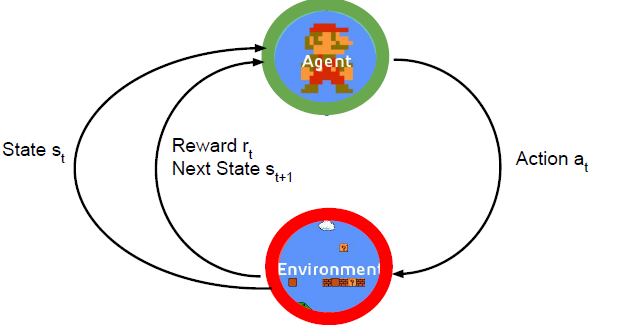
\includegraphics[width=0.7\linewidth]{imgs/chapter13/img0}
			\caption{Reinforcement learning}
			\label{fig:chapter13-00}
		\end{minipage}%
		\begin{minipage}{.5\textwidth}
			\centering
			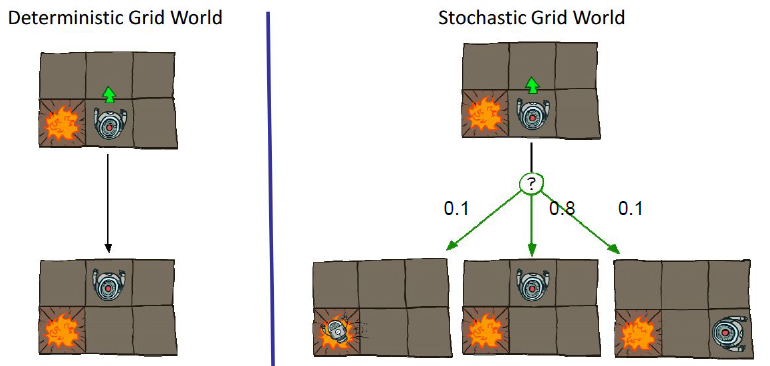
\includegraphics[width=1\linewidth]{imgs/chapter13/img1}
			\caption{Esempi di ambienti}
			\label{fig:chapter13-01}
		\end{minipage}
	\end{figure}
	
	\subsection{MDP loop}
	\begin{itemize}
		\item A tempo $t=0$ l'ambiente si campiona nello stato iniziale $s_0\sim p(s_0)$.
		\item Si ripete:
		\begin{itemize}
			\item L'agente seleziona l'azione $a_i$.
			\item L'ambiente campiona la reward $r_t\sim R(\cdot|s_t, a_t)$.
			\item L'ambiente campiona il prossimo stato $s_{t+1}\sim P(\cdot|s_t, a_t)$
			\item L'agente riceve la reward $r_t$ e lo stato successivo $s_{t+1}$.
		\end{itemize}
	\end{itemize}
	
	\subsection{Policy}
	La policy $\pi(s)$ \`e la funzione da $S$ ad $A$ che specifica quale azione prendere in ogni stato.
	Si deve trovare la policy $\pi^*$ che massimizza cumulative discounted rewards.
	La reward viene data dalla funzione
	$$R:(stato, azione)\rightarrow reward$$

		\subsubsection{Cumulative discounted reward}
		Si supponga di avere una policy $\pi$ in uno stato di inizio $s_0$ che porta a una sequenza $s_0,\dots, s_n$.
		La cumulative reward della sequenza \`e:
		$$\sum\limits_{t\ge 0} r(s_t)$$
		\`E pertanto la somma delle reward di una serie di stati.
		Quella discounted \`e una cumulative reward che d\`a un peso a diverse reward in base al tempo dello step:
		$$\sum\limits_{t\ge 0} y^tr(s_t)\qquad\ where\ 0 < y\le 1$$
		Il discount factor \`e un modo di pesare l'importanza dei primi passi o dei passi futuri in accordo con il valore di $y^t$.
		Minore \`e il discount factor \`e minore l'importanza di reward future e l'agente tende a concentrarsi su azioni che portano a reward immediate.
		Questa strategia aiuta gli algoritmi a convergere.

\section{Confronto tra reinforcement learning e supervised learning}

	\subsection{Supervised learning loop}
	\begin{itemize}
		\item Prendi input $x_i$ campionato dalla distribuzione dei dati.
		\item Utilizza un modello con parametri $w$ per predirre l'output $y$.
		\item Osserva l'output obiettivo $y_i$ e loss $l(w, x_i, y_i)$.
		\item Aggiorna $w$ per ridurre la loss con SGD: $w = w -\eta\nabla l(w, x_i, y_i)$.
	\end{itemize}
	
	\subsection{Reinforcement learning loop}
	\begin{itemize}
		\item Dallo stato $s_i$ svolgi un azione $a$ determinata dalla policy $\pi(s)$.
		\item L'ambiente seleziona lo stato successivo $s'$ in base al modello di transizione $P(s'|s,a)$.
		\item Osserva $s'$ e la reward $r(s)$, aggiornando la policy.
	\end{itemize}
	
	\subsection{Differenze fondamentali}
	\begin{itemize}
		\item Nel SL i dati non dipendono dall'input precedente, mentre in RL le azioni dell'agente influiscono il prossimo input.
		\item In SL si ha una loss function che guida il modello ai parametri migliori e si pu\`o differenziare con rispetto ai pesi, mentre in RL la reward guida lo sviluppo del modello, ma non \`e differenziabile rispetto ai paramatri.
		\item In SL si trova supervisione rispetto ad ogni passo, mentre in RL le rewards potrebbero essere sparse.
	\end{itemize}

\section{Metodi di reinforcement learning}
Per RL si trovano due approcci principali:
\begin{itemize}
	\item Metodi basati sul valore: una value function $V(s)$ viene introdotta e l'agente vuole masssimizzarla.
	La value di ogni stato \`e la quanit\`a totale di reward un agente pu\`o aspettarsi di collezionare rispetto al futuro cominciando da uno stato dato.
	\item Metodo basato sulla policy: si definisce una policy da ottimizzare direttamente, questa definisce come l'agente si comporta nella forma di distribuzione di probabilit\`a tra le azioni da svolgere in uno stato dato.
	Una policy stocastica d\`a la distribuzione di probabilit\`a su azioni diverse: $\pi_\theta(s,a)\approx P(a|s)$.
	
\end{itemize}

	\subsection{Value based methods}
	La funzione di value \`e una funzione dello stato con rispetto a una certa policy $\pi$.
	Ritorna la quantit\`a totale di reward che l'agente pu\`o aspettarsi da uno stato particolare a tutti gli stati possibili a partire da quello.
	Attraverso la value si pu\`o trovare una policy.
	La value function $V$ di uno stato con rispetto a una policy $\pi$ \`e l'aspettata cumulative reward di seguire tale policy cominciando in $s$:
	$$V^\pi(s) = \mathbb{E}\biggl[\sum\limits_{t\ge 0} y^tr(s_t)|s_0 = s,\pi\biggr]$$
	Con $a_t = \pi(s_t), s_{t+1}\sim P(\cdot|s_t, a_t)$.
	Il valore ottimale di uno stato \`e il valore raggiungibile seguendo la migliore policy:
	$$V^*(s) = \max_\pi\mathbb{E}\biggl[\sum\limits_{t\ge 0} y^tr(s_t)|s_0 = s,\pi\biggr]$$
	Dice pertanto quanto \`e buono uno stato.
	Si trova il valore atteso in quanto la sequenza di stati non \`e deterministica e non si ha accesso alla probabilit\`a di transizione.
	Rappresenta il valore che l'agente pu\`o aspettarsi da tutti gli stati possibili cominciando dallo stato iniziale $s$.

		\subsubsection{Q value function}
		Invece di gestire con la value function si utilizza la $Q$-value function che lavora con uno stato $s$, una azione $a$ e una policy $\pi$.
		Viene definita come:
		$$Q^\pi(s,a) = \mathbb{E}\biggl[\sum\limits_{t\ge 0} y^tr(s_t)|s_0 = s,a_0 = a\pi\biggr]$$
		Il valore ottimale di $Q$ dice quando \`e buona una coppia stato azione:
		$$Q^*(s,a) =\max_\pi\mathbb{E}\biggl[\sum\limits_{t\ge 0} y^tr(s_t)|s_0 = s,a_0 = a\pi\biggr]$$
		La Q value ottimale viene usata per computare la policy ottimale:
		$$\pi^*(s) = arg\max_aQ^*(s,a)$$
		La formula risultate della $Q$ value function \`e nella formula di un'equazione di Bellman:
		\begin{align*}
			Q^*(s,a) &= r(s) + y\sum\limits_{s'}P(s'|s,a)\max_{a'}Q^*(s',a')\\
			&=\mathbb{E}_{s'\sim P(\cdot|s,a)}[r(s)+y\max_{a'}Q^*(s',a')|s,a]
		\end{align*}
		Se il valore ottimale della coppia stato azione per il prossimo passo $Q^*(s',a')$ sono conosciuti allora la strategia ottima \`e svolgere l'azione che massimizza il valore atteso.
		Per calcolare il valore $Q$ dello stato corrente si deve calcolare il valore $Q$ degli stati vicini e cos\`i via con ricorsione.
		
		\subsubsection{Algoritmo Q-learning}
		Lo scopo di questo algoritmo \`e che la matrice di value $R$ \`e conosciuta unicamente all'ambiente e l'agente deve impararla con l'esperienza.
		L'agente possiede una matrice $Q$ che codifica stato, azione e rewards, ma \`e inizializzata a $0$ e diventa $R$ attraverso l'esperienza.
		La policy si ottiene attraverso questa matrice.
		\begin{enumerate}
			\item Inizializza la matrice $Q$ con zero.
			\item Seleziona uno stato iniziale casuale.
			\item Per ogni episodio (insieme di azioni che parte dallo stato iniziale e arriva allo stato finale).
			\item Mentre lo stato non \`e lo stato obiettivo.
			\item Seleziona una possibile azione casuale per lo stato corrente.
			\item Utilizzando l'azione considera arrivare allo stato prossimo.
			\item Ottieni il valore di $Q$ massimo per il prossimo stato.
			\item $Q^*(s,a) = R(s,a)+y\max\limits_a[Q^*(s',a')]$.
		\end{enumerate}
		Per trovare la policy ottimale:
		\begin{enumerate}
			\item Si pone lo stato corrente a quello iniziale.
			\item Dallo stato corrente si trova l'azione con il maggiore $Q$ value.
			\item Si pone lo stato corrente al prossimo.
			\item Si ripetono i passi $2$ e $3$ fino a che si raggiunge lo stato obiettivo.
		\end{enumerate}

		\subsubsection{Deep Q learning}
		L'equazione di Bellman pu\`o pertanto essere usate per imparare tabelle $Q$ per ritornare la policy ottimale.
		Nel mondo reale per\`o gli stati e le rewards possono essere troppo grandi per essere calcolate completamente.
		Per questa ragione viene introdotto un algoritmo di deep $Q$ learning che sfrutta l'idea di approssimare $Q$ utilizzando una funzione parametrica trainata da una NN.
		Si pu\`o approssimare $Q$ a
		$$Q^*(s,a) \approx Q_w(s,a)$$
		In quanto $Q_w$ \`e una funzione dei pesi $w$ si pu\`o trainare una NN per approssimare $Q_w$.
		Ad ogni interazione del training si aggiornano i parametri $w$ del modello per avvicinare $Q$ a $y$:
		$$y_i(s,a) = \mathbb{E}_{s'\sim P(\cdot|s,a)}[r(s)+y\max_{a'}Q_{w_{i-1}}(s',a')|s,a]$$
		La loss function
		$$L_i(w_i) = \mathbb{E}_{s,a\sim \rho}[(y_i(s,a) - Q_{w_i}(s,a))^2]$$
		Dove $\rho$ \`e la distribuzione di probabilit\`a sugli stati $s$ e le azioni $a$ che si riferiscono come distribuzione di comportamento.
		Si definisce a ogni iterazione $i$ e un target $y_i$ ottenuti attraverso la Bellman equation.
		Dati questi valori si pu\`o derivare $L_i$.
		Aggiornamento del gradiente:
		\begin{align*}
			\nabla_{w_i}L(w_i) &= \mathbb{E}_{s,a\sim\rho}[(y_i(s,a) - Q_{w_i}(s,a))\nabla_{w_i}Q_{w_i}(s,a)]=\\
			&= \mathbb{E}_{s,a\sim\rho,s'}[(r(s) + y\max_{a'}Q_{w_{i-1}}(s',a')-Q_{w_i}(s,a))\nabla_{w_i}Q_{w_i}(s,a)]
		\end{align*}
		Attraverso il training SGD si sostituisce il valore atteso campionando l'esperienza $(s,a,s')$ utilizzando la distribuzione di comportamento e il modello di transizione.
		
		\paragraph{Problematiche}
		Il training \`e prono all'instabilit\`a e a differenza del supervised learning i target si muovono.
		Esperienze successive sono correlate e dipendenti dalla policy che pu\`o cambiare rapidamente con piccoli cambi nei parametri, portando a un cambio drastico nella distribuzione dei dati.
		Per risolverli si pu\`o fare freezing sulla target Q network per aumentare la stabilit\`a della rete e utilizzare un experience replay: un buffer per salvare esperienze e campionare da quello in modo da seguire una strategia greedy che permette un trade-off tra exploitation ed esploration.

	\subsection{Policy gradient methods PGM}
	L'obiettivo dei PGM \`e di definire parametri che influenzano la policy $\pi$ e di impararli direttamente.
	Questa \`e la soluzione pi\`u semplice nel caso in cui si abbia uno spazio degli stati grande e continuo.
	L'idea \`e di utilizzare deep neural network per imparare la policy.
	Si deve pertanto imparare una funzione che ritorna la distribuzione di probabilit\`a di azioni rispetto allo stato corrente:
	$$\pi_\theta(s,a)\approx P(a|s)$$
	Si noti come questa ha un significato diverso rispetto ai value-based method: \`e una probabilit\`a di azioni rispetto agli stati, non una funzione da azioni a stati.
	In questo caso non si hanno le labels in modo da dare feedback alla NN attraverso backpropagation e viene usata la reward.
	Si devono pertanto trovare i migliori parametri $\theta$ della policy per massimizzare la reward aspettata attraverso gradient descent:
	\begin{align*}
		J(\theta) &= \mathbb{E}\biggl[\sum\limits_{t\ge 0}y^tr_t|\pi_\theta\biggr]\\
		&=\mathbb{E}_\tau[r(t)]
	\end{align*}
	Si vuole il valore atteso di ritorno di traiettorie: $\tau(s_0,a_0,r_0, \dots, s_n,a_n,r_n)$
	$$J(\theta) = \int_\tau r(\tau)p(\tau,\theta)d\tau$$
	Dove $p(\tau,\theta)$ \`e la probabilit\`a della traiettoria $\tau$ sotto la policy con i parametri $\theta$:
	$$p(\tau,\theta) = \prod\limits_{t\ge 0}\pi_\theta(s_t,a_t)P(s_{t+1}|s_t,a_t)$$
	Le traiettorie sono una semplificazione, un oggetto che rappresenta stato, azione e reward.
	In quanto l'integrale \`e di difficile risoluzione si differenzia utilizzando la log-trasformation:
	$$\nabla_\theta J(\theta) =\mathbb{E}_\tau[r(t)\nabla_\theta\log p(\tau,\theta)]$$
	Dove
	$$\log p(\tau,\theta) = \sum\limits_{t\ge 0} [\log \pi_\theta(s_t,a_t) + \log P(s_{t+1}|s_t,a_t)]$$
	E
	$$\nabla_\theta \log p(\tau,\theta) = \sum\limits_{t\ge 0}\nabla_\theta \log\pi_\theta(s_t,a_t)$$
	In questo modo si pu\`o computare il gradiente senza conoscere la probabilit\`a di transizione $p$.
	$$\nabla_\theta J(\theta) = \mathbb{E}_\tau\biggl[\biggl(\sum\limits_{t\ge 0}y^tr_t\biggr)\biggl(\sum\limits_{t\ge 0}\nabla_\theta\log\pi_\theta(s_t,a_t)\biggr)\biggr]$$
	Si pu\`o inoltre evitare di computare tutte le traiettorie possibili e usare unicametne un'approssimazione stocastica a $N$ traiettorie.
	$$\nabla_\theta J(\theta) \approx \dfrac{1}{N}\sum\limits_{i=1}^n\biggl(\sum\limits_{t = 0}^{T_i}y^tr_{i,t}\biggr)\biggl(\sum\limits_{t= 0}^{T_i}\nabla_\theta\log\pi_\theta(s_{i,t},a_{i,t})\biggr)$$

		\subsubsection{Reinforce}
		Reinforce \`e un algoritmo per deep RL che aggiorna i parametri:
		\begin{enumerate}
			\item Campiona $N$ traiettorie $\tau_i$ utilizzando la policy corrente $\pi_\theta$.
			\item Stima il gradiente di policy $\nabla_\theta J(\theta)$.
			\item Aggiorna i parametri attraverso gradient ascent $\theta = \theta + \eta\nabla_\theta J(\theta)$.
		\end{enumerate}
		
		\subsubsection{Single step reinforce}
		Single step reinforce \`e una variante del reinforce che stima il gradiente unicamente su uno step e non sull'intera traiettoria:
		\begin{enumerate}
			\item In uno stato $s$ campiona l'azione $a$ utilizzando la policy corrente $\pi_\theta$ e si osserva la reward $r$.
			\item Stima il gradiente $\nabla_\theta J(\theta)\sim r\nabla_\theta\log\pi_\theta(s,a)$
			\item Aggiorna i parametri attraverso gradient ascent $\theta = \theta + \eta\nabla_\theta J(\theta)$.
		\end{enumerate}
		Si nota come $r$ alto aumenta la probabilit\`a dell'azione vista, mentre se \`e basso si abbassa la probabilit\`a.
		Si aggiorna il parametri $\theta$ in accordo con il gradiente in quanto si vuole aumentare la reward o gradient ascent.
